\documentclass[11pt,oneside]{amsart}
\usepackage{geometry}
\usepackage[T1]{fontenc}
\usepackage{lmodern}
\usepackage{booktabs,pdfpages,parskip}

\newcommand{\eps}{\varepsilon}
\newcommand{\bE}{\mathbb{E}}
\DeclareMathOperator{\Var}{Var}

\pagestyle{empty}

\title{Instructor's Report, Fall 2022\\ \today}

\begin{document}
\maketitle

\bigskip

\textbf{Course number, name:} MATH1103, Calculus II (Math/Science Majors)

\textbf{Instructor:} Yongyi Chen

\section{Report}
\subsection{Texts}
\begin{itemize}
  \item Gilbert Strang's \emph{Calclus} for integration
  \item Mark Reeder's in-house MATH1103 notes for integration and series.
\end{itemize}

\subsection{Topics (include sections of text)}
Each bullet point at level 2 represents one week of class.
\begin{itemize}
  \item Integration and applications
        \begin{itemize}
          \item History, areas, definition of definite integral, properties of definite integral, indefinite integrals (Strang 5.1, 5.2, 5.3, 5.5, 5.6)
          \item Fundamental theorem of calculus I and II, $u$-substitution (Reeder 9.5, 9.7, 9.9; Strang 5.4, 5.7)
          \item Integration by parts, trig substitution (Strang 5.4, 7.1, 7.2; Reeder 9.8, 9.9)
          \item Expected value, basic probability, areas, volumes (Strang 5.6, 8.1; Reeder 9.15)
          \item Arc length, surface area, advanced probability (Strang 8.2, 8.3, 8.4; Reeder 9.13, 9.12)
          \item More advanced probability (Strang 8.4, Reeder 9.12)
          \item Improper integrals and proof that $\pi$ is irrational (Strang 7.5, Niven)
        \end{itemize}
  \item Sequences and series
        \begin{itemize}
          \item Intro to sequences, the $\eps$-lemma, the $\eps$ definition of convergence (Reeder 1)
          \item More work on the $\eps$ definition, intro to series (Reeder 1, 3)
          \item Geometric series (Reeder 3)
          \item Comparison theorem and other convergence tests (Reeder 3)
          \item Power series (Reeder 4)
        \end{itemize}
  \item Additional topics
        \begin{itemize}
          \item Proof that $e$ is irrational, combining power series and integration, for example representing erf values as an infinite series that converges very fast.
        \end{itemize}
\end{itemize}

\subsection{Some comments about the text}

\subsubsection{Strang's textbook}
The textbook is very well organized. In my opinion it has excellent exposition, motivation, and examples, although I find that most students do not attempt to read the exposition and only prefer to read their handwritten notes (a learned habit from their pre-college math education no doubt). It may be that school does not adequately teach them the level of mathematical maturity required to learn from the exposition. The exercises and problems at the end of each section had excellent variety and challenge, and I drew from them a lot when designing my problem sets.

I also very much liked the way Strang presented the probability section.

\subsubsection{Reeder's notes}
Mark Reeder's MATH1103 notes were excellent too. The flow of topics was non-traditional but, in my opinion, much better motivated than, say, Stewart's. However, I found that the students' schooling did not teach the students enough mathematical maturity to fully absorb the rigorous mathematical language in the notes, so I frequently had to adapt the content to their level of mathematical rigor. This is not a drawback of the notes themselves by any means; one could say the students are not adequately prepared to fully absorb any heavy logical content (such as proofs) that would appear in any calculus textbook.

The notes themselves do not contain many exercises or problems but Mark Reeder graciously provided me with his old homework which I could draw problems from. The problems were excellent, as well.

It's important to note that Reeder's notes are intended for a series-first approach to calculus, and since I was asked to take the integration-first approach, I had to select a different text for the integration part of the course due to the heavy integration of power series in Reeder's integration chapters. As I already mentioned, Strang was my choice.

% \subsubsection{Why I didn't use Stewart}
% I chose to avoid Stewart's textbook not because of anything about the textbook itself, but because I predicted, based on my experience from last year in MATH1101, that having Stewart as a textbook would signal to students that we would be doing ``more of the same'' kind of ``mathematics'' that they learned in high school. The most prominent feature of this kind of ``mathematics'' is learning by identifying problem types and executing a procedure learned for that problem type. 

\subsection{Course format}
In-person, one-hour lectures 3 times per week. Weekly problem sets, with one multi-part (6-8 parts) problem for skill practice and then 2 to 4 challenging problems. In these problem sets, full solutions were expected to be written up. No online homework. According to course evaluations, students still spent on average around 6--9 hours per week on homework, which is higher than the school average.

\subsection{Number of exams}
Two midterm exams (50 minutes) and one final exam (3 hours). All were done in person, and all were open notes.

\subsection{Enrollment}
\begin{itemize}
  \item Section 1: 19 (plus 1 listener).
  \item Section 2: 12.
  \item Total: 31 (plus 1 listener).
\end{itemize}
(This semester saw 0 late drops or withdrawals.)

\subsection{Grading policy}
\begin{itemize}
  \item 20\% homework,
  \item 20\% first exam,
  \item 20\% second exam,
  \item 40\% final.
\end{itemize}
Each exam was designed so that half of it is skill-based and the other  half is problem solving-based. I designed the difficulty of the problems so that scoring 50\% of the possible points indicates B level performance and scoring 75\% of the possible points indicates A level performance. This may seem like an extreme curve but this is because my exam problems were designed to push the students' thinking.

On the second midterm and final, I gave the instruction to write down partial progress and failed solution attempts for partial credit. I now think this is a very good idea.

Each homework problem was graded on a scale of 0--3 points. I think this is also a very good idea. It may seem like the coarse scale gives students permission to be sloppy with their work but, counterintuitively, that was not the case at all! They still put their best work into the problems. So in some sense, this is a small example of ``ungrading.''

\subsection{General comments about this course}
There was a serious challenge I had to tackle in this class, but by the end it was a big success. First, the successes:
\begin{itemize}
  \item The lectures, homework, and exams in the course ended up being very cohesive and there was a clear sense of mathematical story throughout the semester. Moreover, students were unanimously happy (as far as I can tell, at least) about the the grading of the homework and exams.
  \item Students enjoyed the challenging problems and even called them fun, although some initially complained that they had trouble starting them.
  \item Students liked the historical approach in Reeder's notes, especially seeing how mathematicans such as Euler contributed to calculus. It really showed them that math is a lively human endeavor, not a cold subject. In fact, after showing how Euler proved that $\sum_{n=1}^\infty 1/n^2=\pi^2/6$ using an infinite product expansion of $\sin x$, two students were extremely eager and wondered what would happen if you look at $\cos x$ instead. They worked it out in my office hours all by themselves and got $\sum_{n=0}^\infty 1/(2n+1)^2=\pi^2/8$. Amazing! And this was just one of many examples of students being excited about mathematics.
  \item Also thanks to Reeder's notes, students were very quick to understand the nature of a mathematical proof and what a proof is. I have not heard a single expression of fear of the word ``proof'' in this class, and the proof questions on exams had high success rates.
  \item After the interventions I made mid-semester (described below), performance on exams rose drastically, from 60\% average on the first exam to 80\% average on the second exam and 73\% average on the final. I think the performance on the final is especially impressive given the problems I put on there -- the last four problems on the final consisted entirely of problems that were new to them to some extent.
\end{itemize}
Now onto the challenges. The main challenge was finding out after the first exam that about half of the students were not picking up on the habits of mathematical thinking even though I demonstrated them during lectures and had them practice them by doing challenging homework problems. By mathematical thinking here, I do not mean something as advanced as proof skills required of math majors, but something like the following:
\begin{itemize}
  \item The ability to apply knowledge to a new context.
  \item The ability to start a problem for which the solution is not known in advance.
  \item The ability to make logical deductions from previous work and knowledge. (A Chinese phrase that Yaoying taught me that is about this is the Confucian saying ``ju yi fan san,'' meaning ``learn one, deduce three.'')
\end{itemize}
These three skills are absolutely crucial in every walk of life. They are also required if you want students to have a true understanding of the material in any math class (especially the skill of making logical deductions, aka ``ju yi fan san'').

% Of course, I had expected that students would have little training in mathematical thinking based on my experiences in MATH1101 last year. This is despite the fact that Common Core has been around for 12 years, and mathematical thinking is heavily emphasized in the Common Core in its 8 Standards of Mathematical Practice. I even asked the MATH1103 students on day 2 the following question:
% \begin{quote}
%   How many of you were taught math by learning problem types and procedures to solve each problem type?
% \end{quote}
% And every single student in both sections raised their hand, to my amazement. I then told them that what they would be doing in this class is not this. Evidently just telling them that proved to not be enough.

After a lot of thinking, I came up with the following three reasons why students did not gain mathematical thinking habits by mid-semester:
\begin{itemize}
  \item Many students complained that they could not start the challenging problems and needed to get help. After getting help, they were able to proceed. But maybe the help they got was too guided and they failed to generalize their lessons.
  \item Most students thought lectures were meant to be pure informational material (to be copied down).
  \item Lecture is ineffective in changing habits, namely the (non)-problem solving habits they learned in school. Even doubly so if they are just writing things down during lectures without thinking.
\end{itemize}

I made several interventions in response to this. They are as follows:
\begin{itemize}
  \item On each homework, I started asking them to rate the difficulty of each homework problem on a 1--7 scale (you can see in the attached homeworks), with 6--7 representing that had to seek help and still don't understand the problem afterwards. This benefitted me in that I could see which homework problems they struggled on, and also benefitted them in knowing which homework problems to redo when it came time to study for exams.
  \item In order to teach them how to start a novel problem, I spent significant class time calling groups of 4 at a time to the board to start problems by writing down observations and logical deductions. It is important to note that this is not the same as ``groupwork,'' in fact I did not ask them to finish the problem (although many groups did manage to finish the problem).
\end{itemize}
It is interesting to note that the second item not only teaches how to start a problem but also has the effect of slowing down the pace of the lectures (a good thing for students who are struggling to keep up) as well as allowing students to show different approaches for a problem to the whole class.

\subsubsection{Yaoying's comments}
Yaoying has told me that often in discussions, students would sit and stare at the discussion questions until Yaoying comes to help. When this is the case, a compromise must be struck between helping students individually and helping the class as a whole. This is another case where it's clearly better if students were taught how to start on problems before entering college!

% \subsubsection{Some more details}
% For example, despite having used integrals to prove that $\Var(X)=\bE[X^2]-\bE[X]^2$ on their most recent problem set, and having this equation given to them on the exam, many of the students were unable to go backwards and turn the equation into integrals to find the variance of an exponential distribution.

% To be honest, if I would like discussions to be more effective, having them work together first is a good idea — however, some are willing to do so while some are not. For those who don’t work with others, they simply sit there and look at the questions and then stare at them, stare at them….. until I came up to help. Then the question is, if I spend too much time on helping one student, I’ll definitely be running out of time. If I don’t do so, I cannot make sure students like that get how much from the class! So, maybe striking a balance and finding some better ways to get everybody started to work would be something I’d like to figure out as well😂😂😂


\subsection{Final grade distribution}
\begin{itemize}
  \item 16 A
  \item 4 A$-$
  \item 4 B$+$
  \item 3 B
  \item 2 B$-$
  \item 2 C$+$
\end{itemize}


\vskip 0pt plus 1fill minus 0pt
\noindent
\textbf{Attached are the syllabus, all tests (including final), list of
  HW assignments, and any other pertinent material.}
\newpage

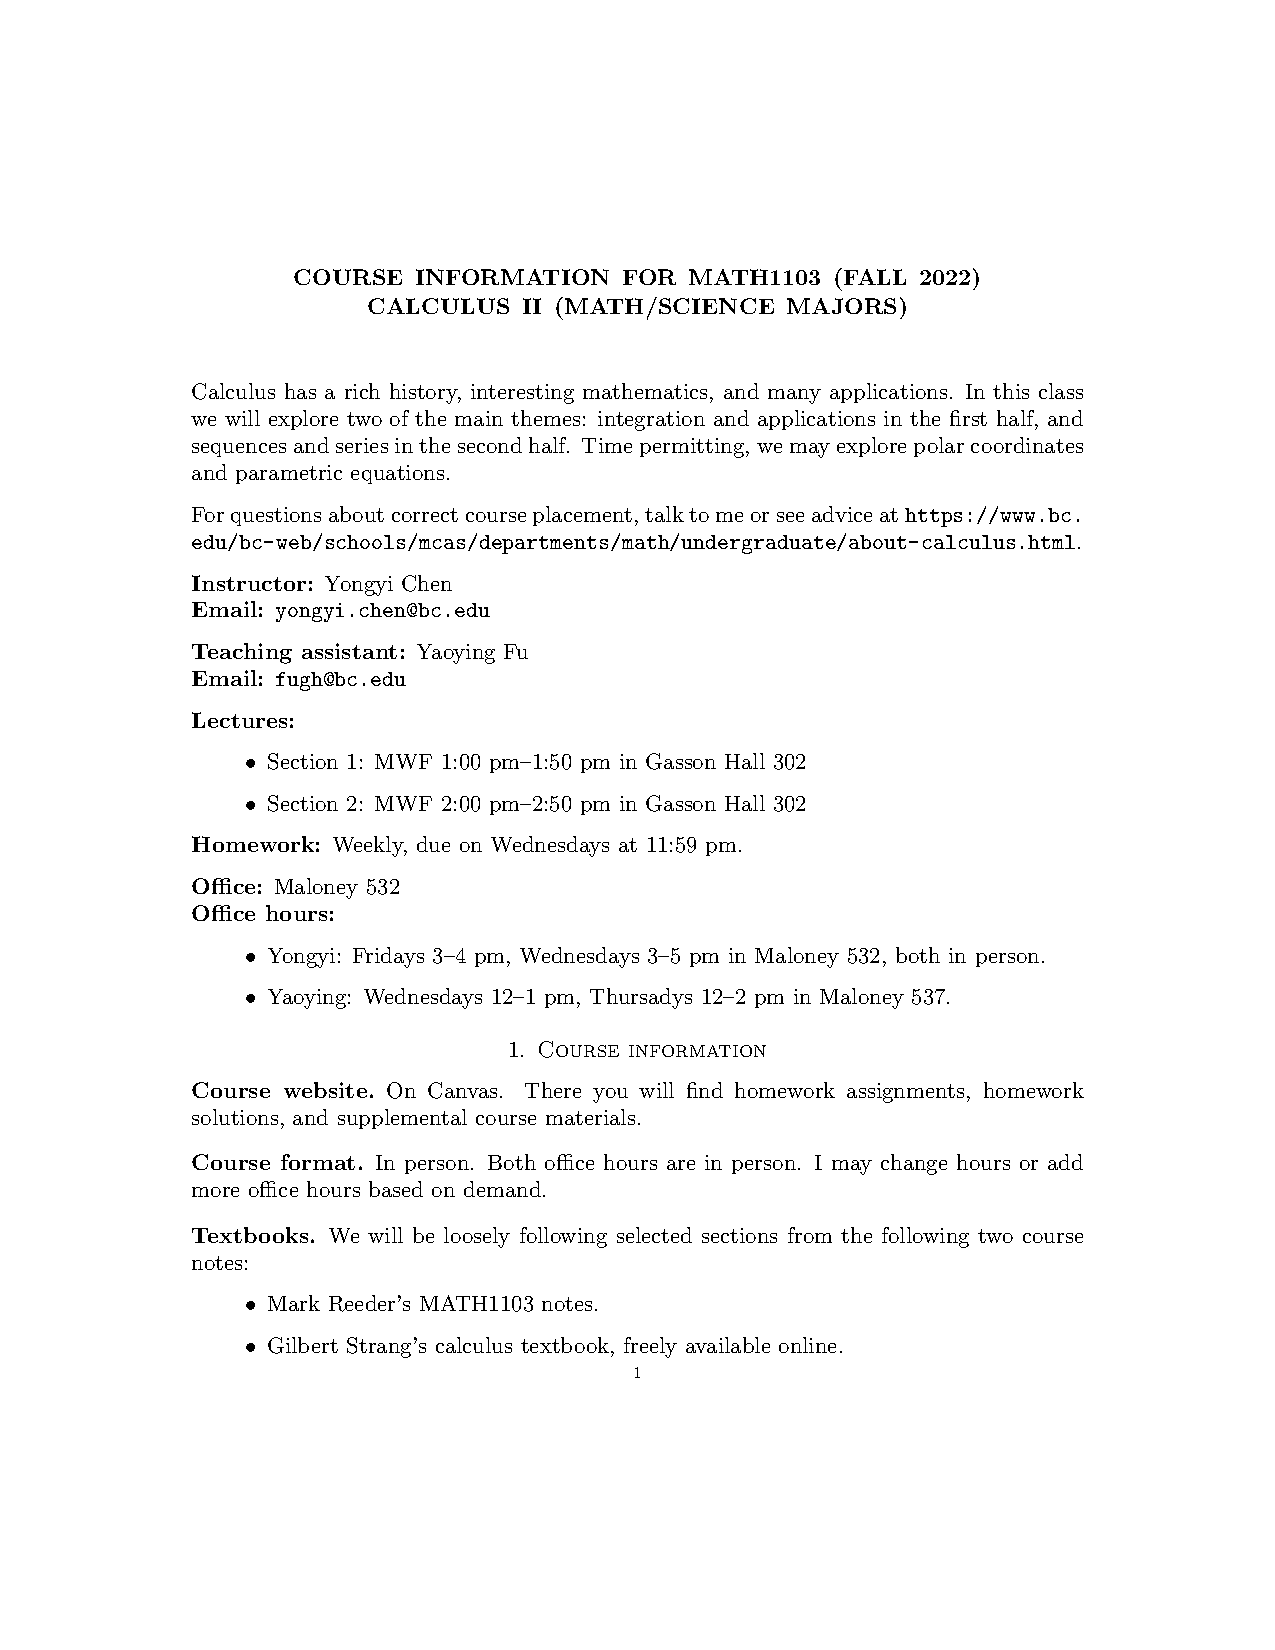
\includepdf[pages=-]{syllabus.pdf}
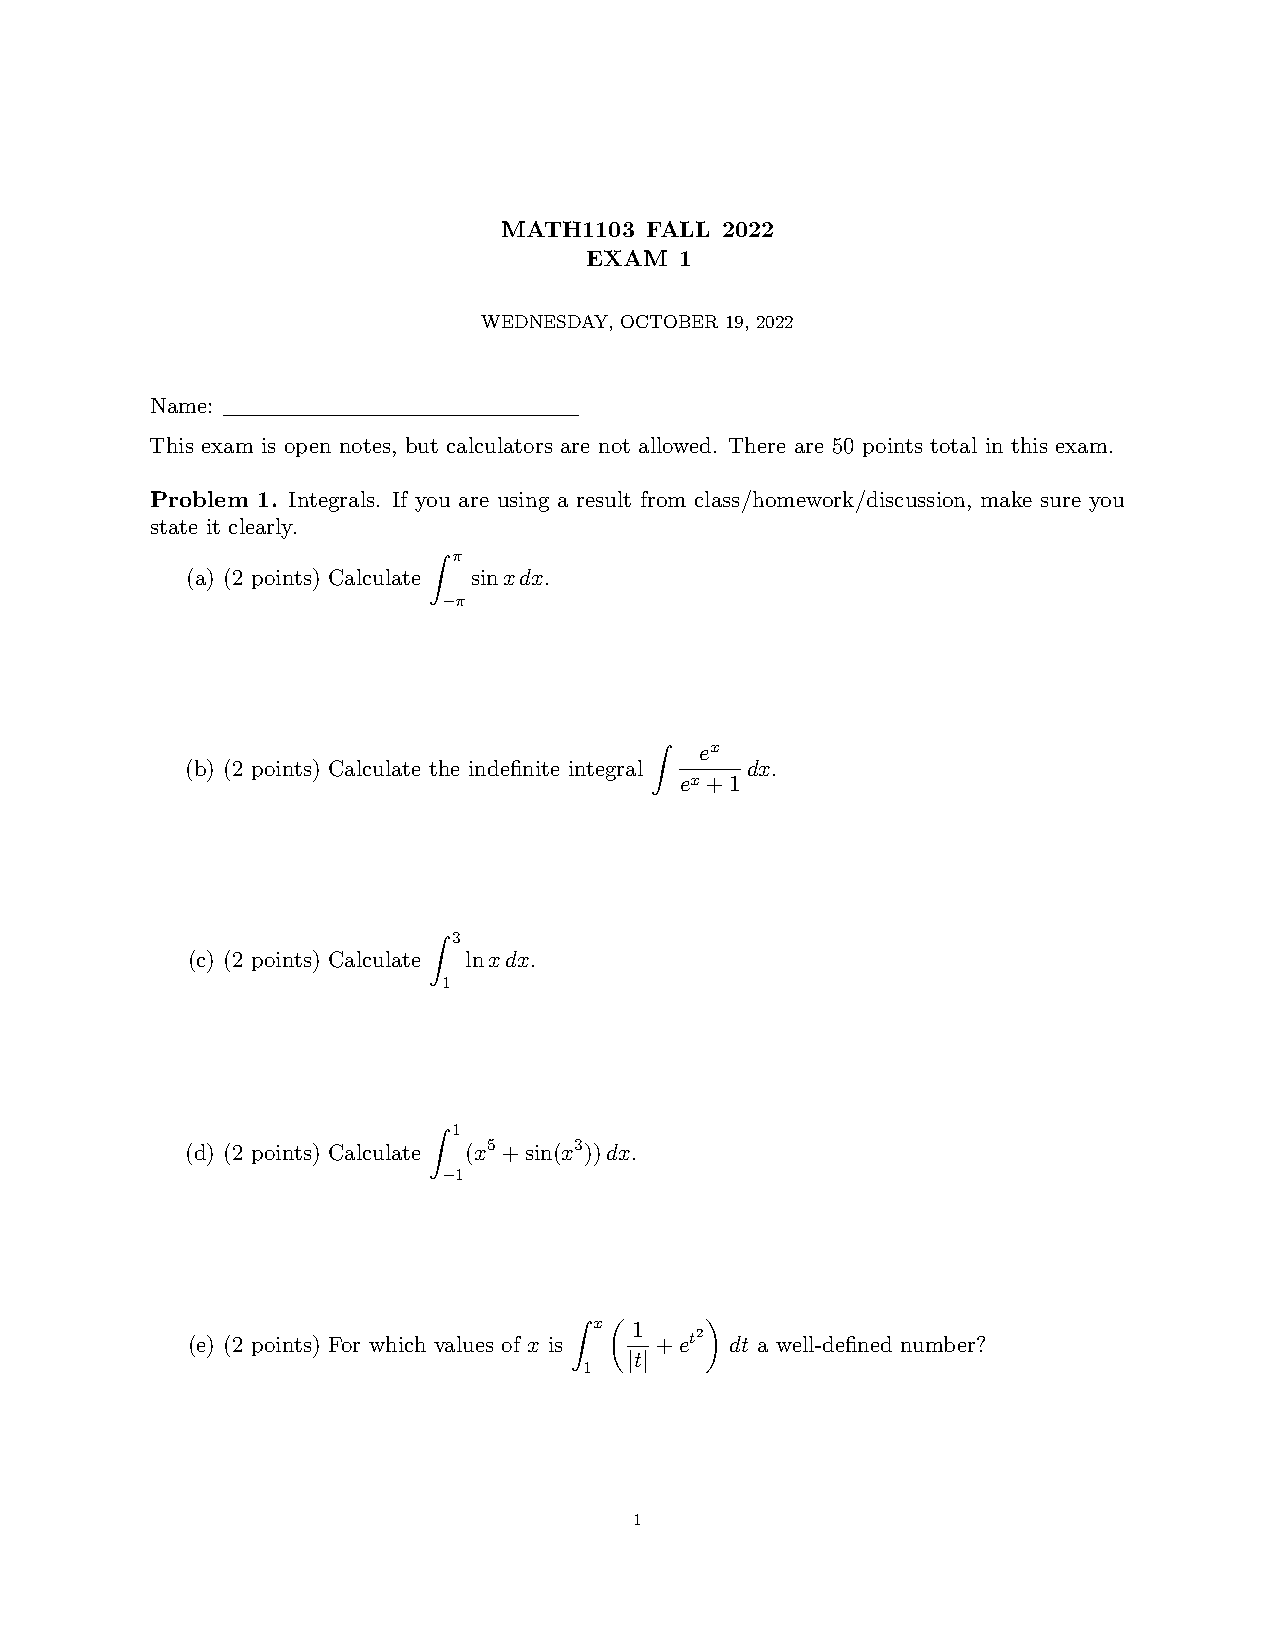
\includepdf[pages=-]{exam1/exam1.pdf}
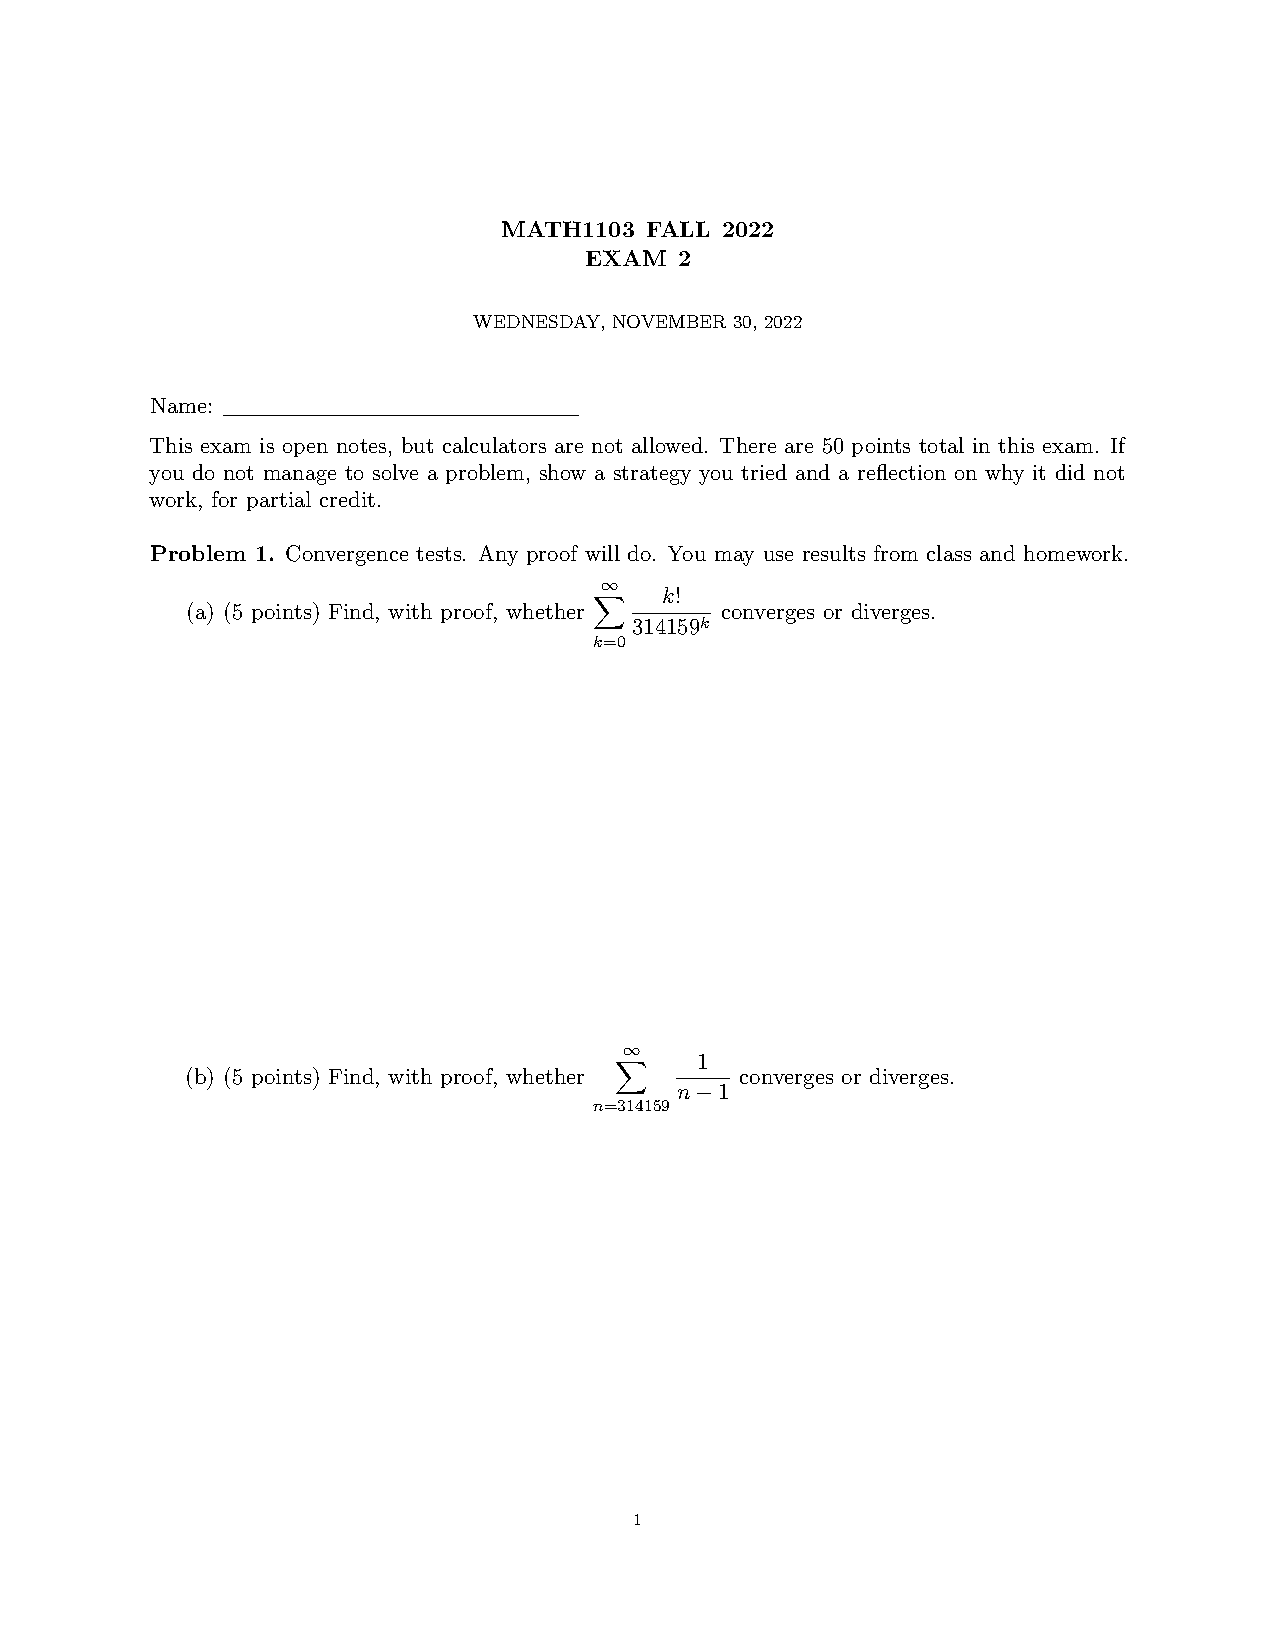
\includepdf[pages=-]{exam2/exam2.pdf}
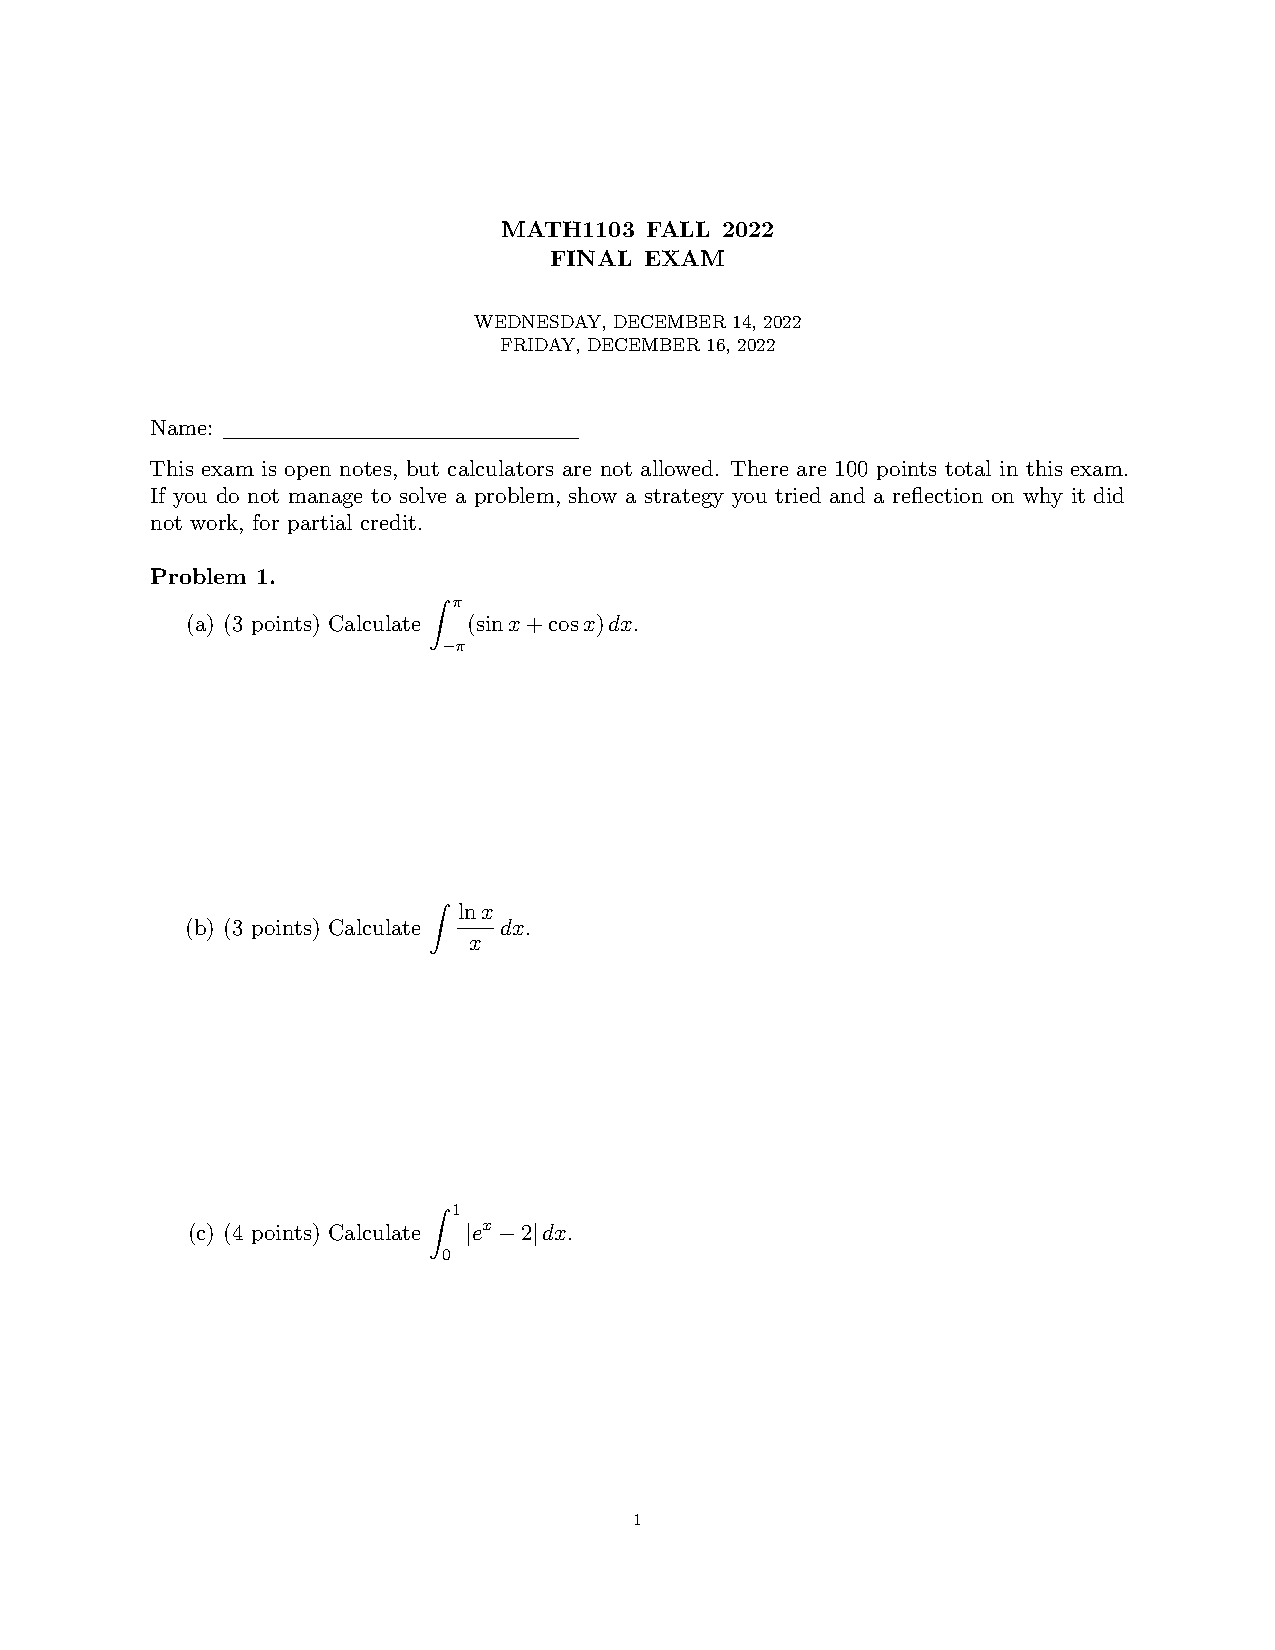
\includepdf[pages=-]{final_exam/final_exam.pdf}

% Attach psets 1 through 10.5.
\newcounter{int}
\setcounter{int}{1}
\loop
\includepdf[pages=-]{pset\theint/pset\theint.pdf}
\addtocounter{int}{1}
\ifnum \value{int}<11
\repeat
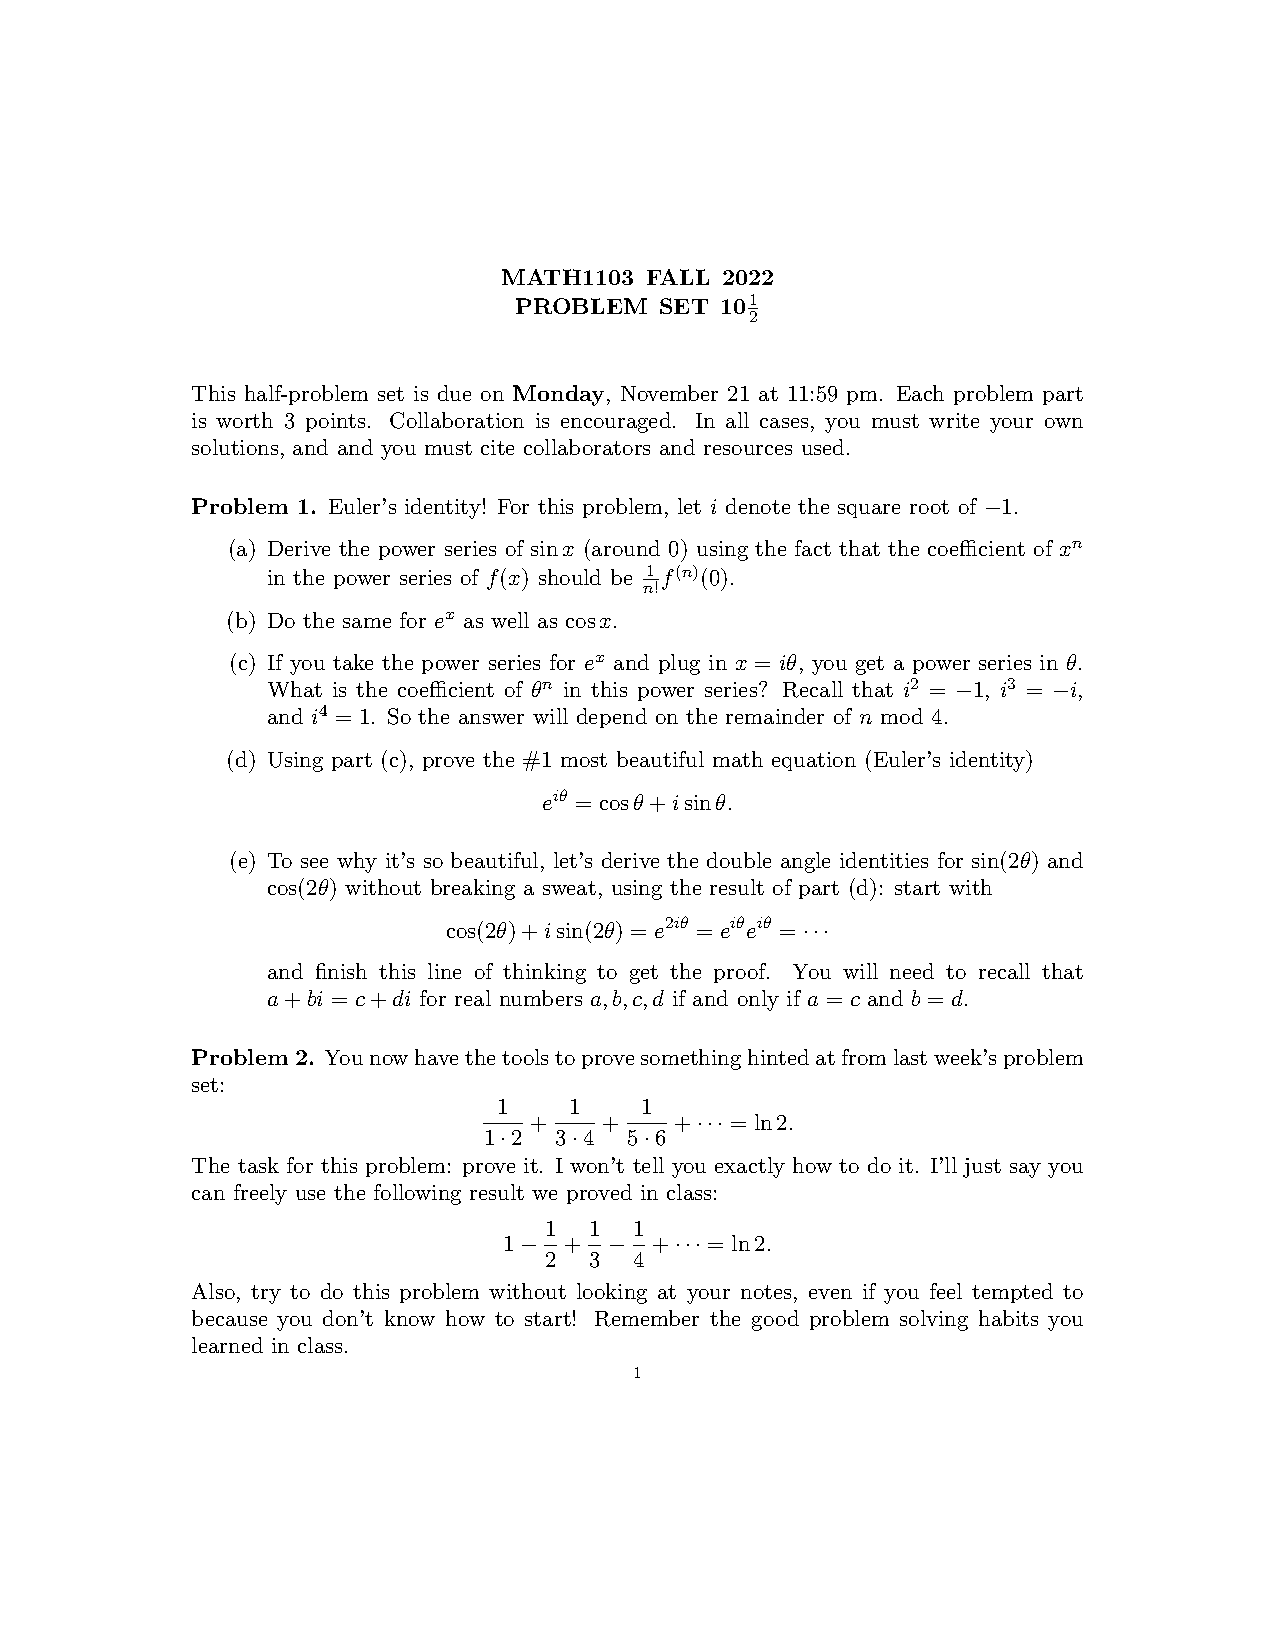
\includepdf[pages=-]{pset10.5/pset10.5.pdf}
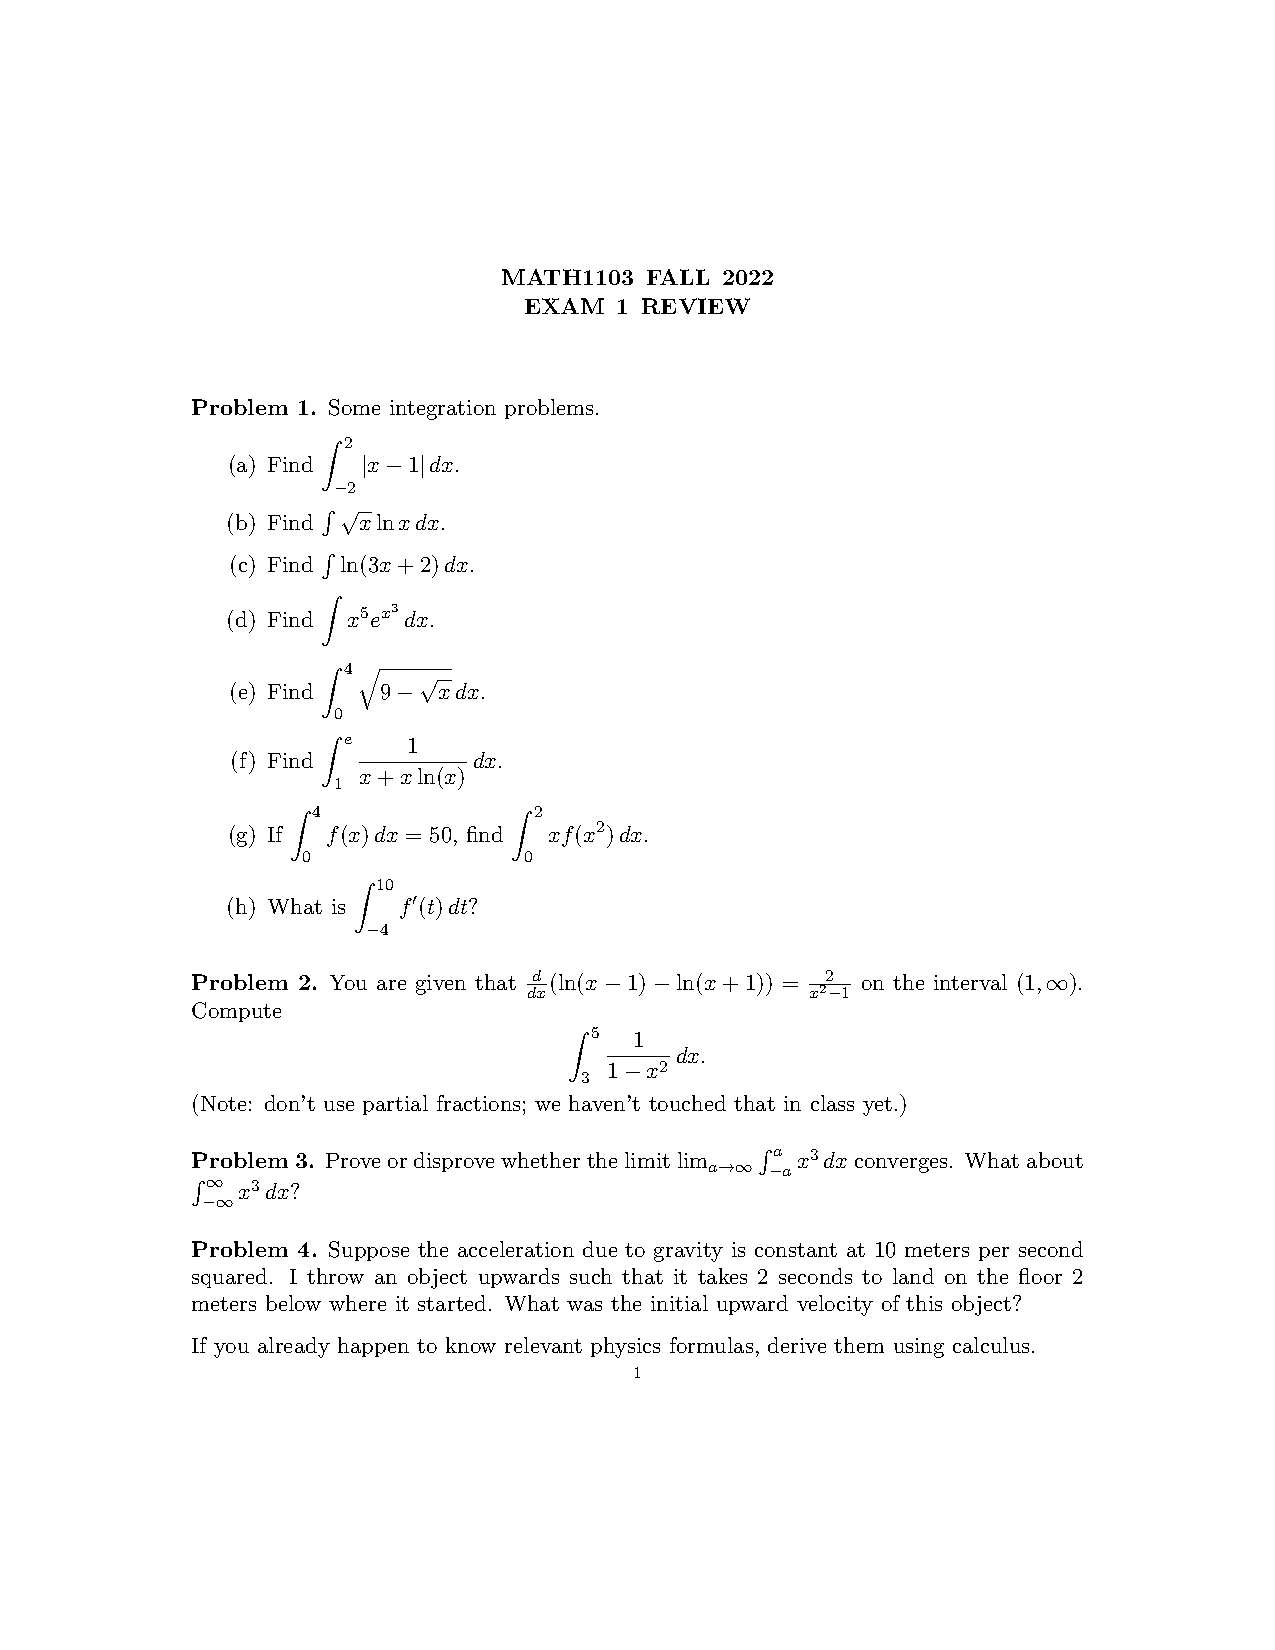
\includepdf[pages=-]{exam1/review1.pdf}
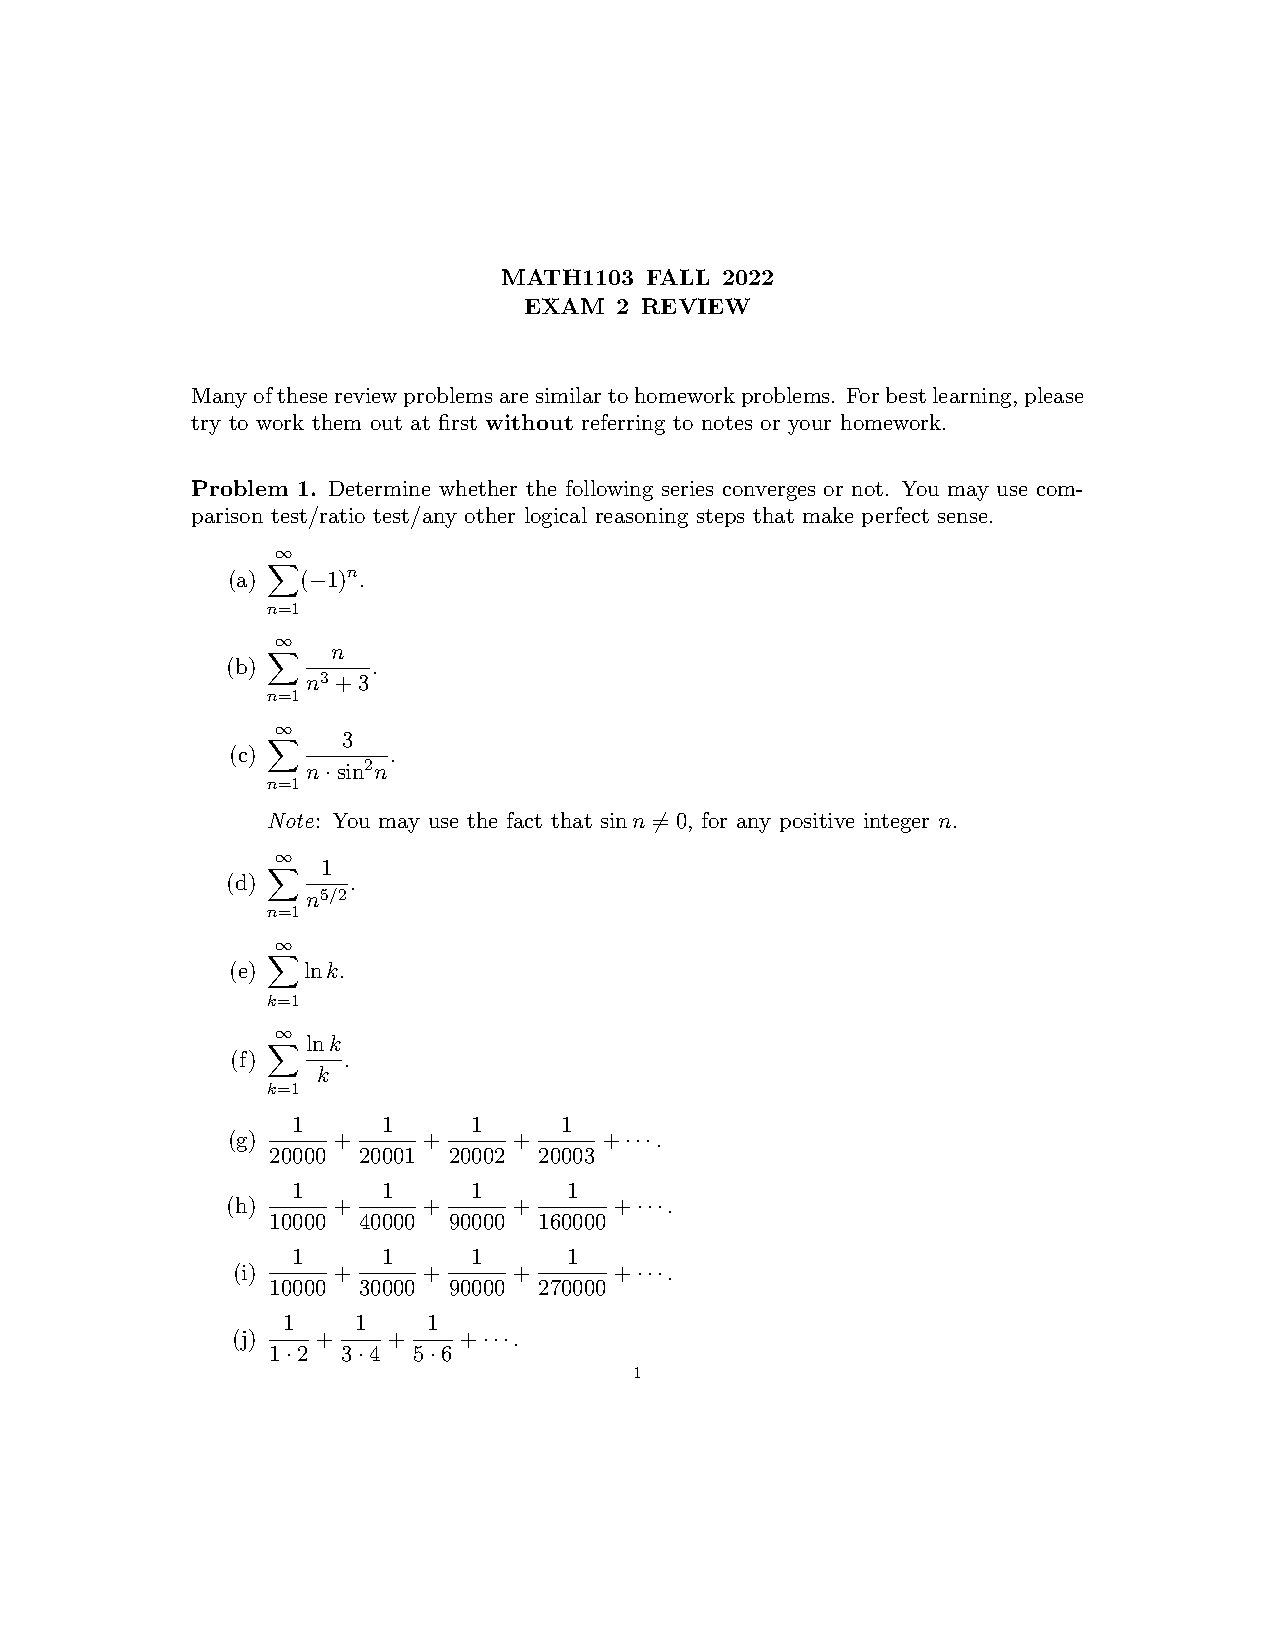
\includepdf[pages=-]{exam2/review2.pdf}
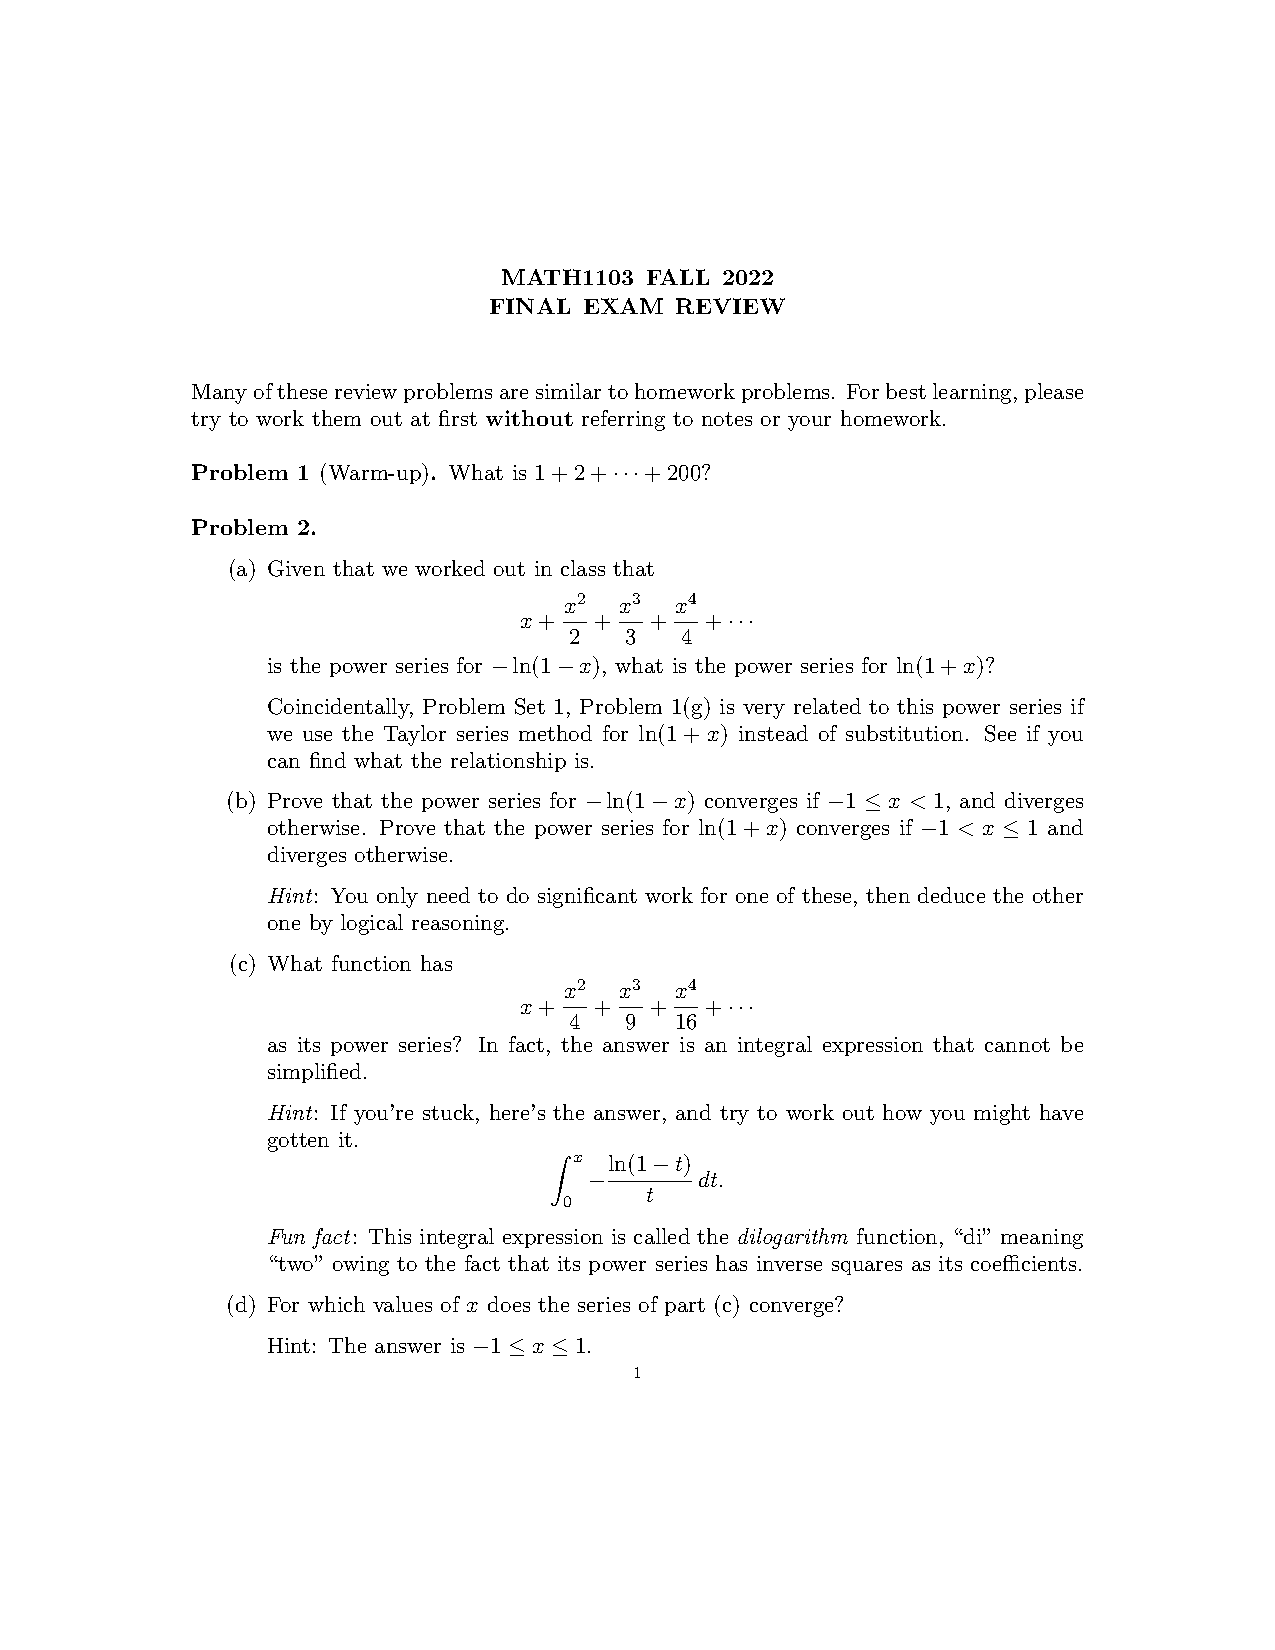
\includepdf[pages=-]{final_exam/final_review.pdf}

\appendix
\section{Supplementary materials}
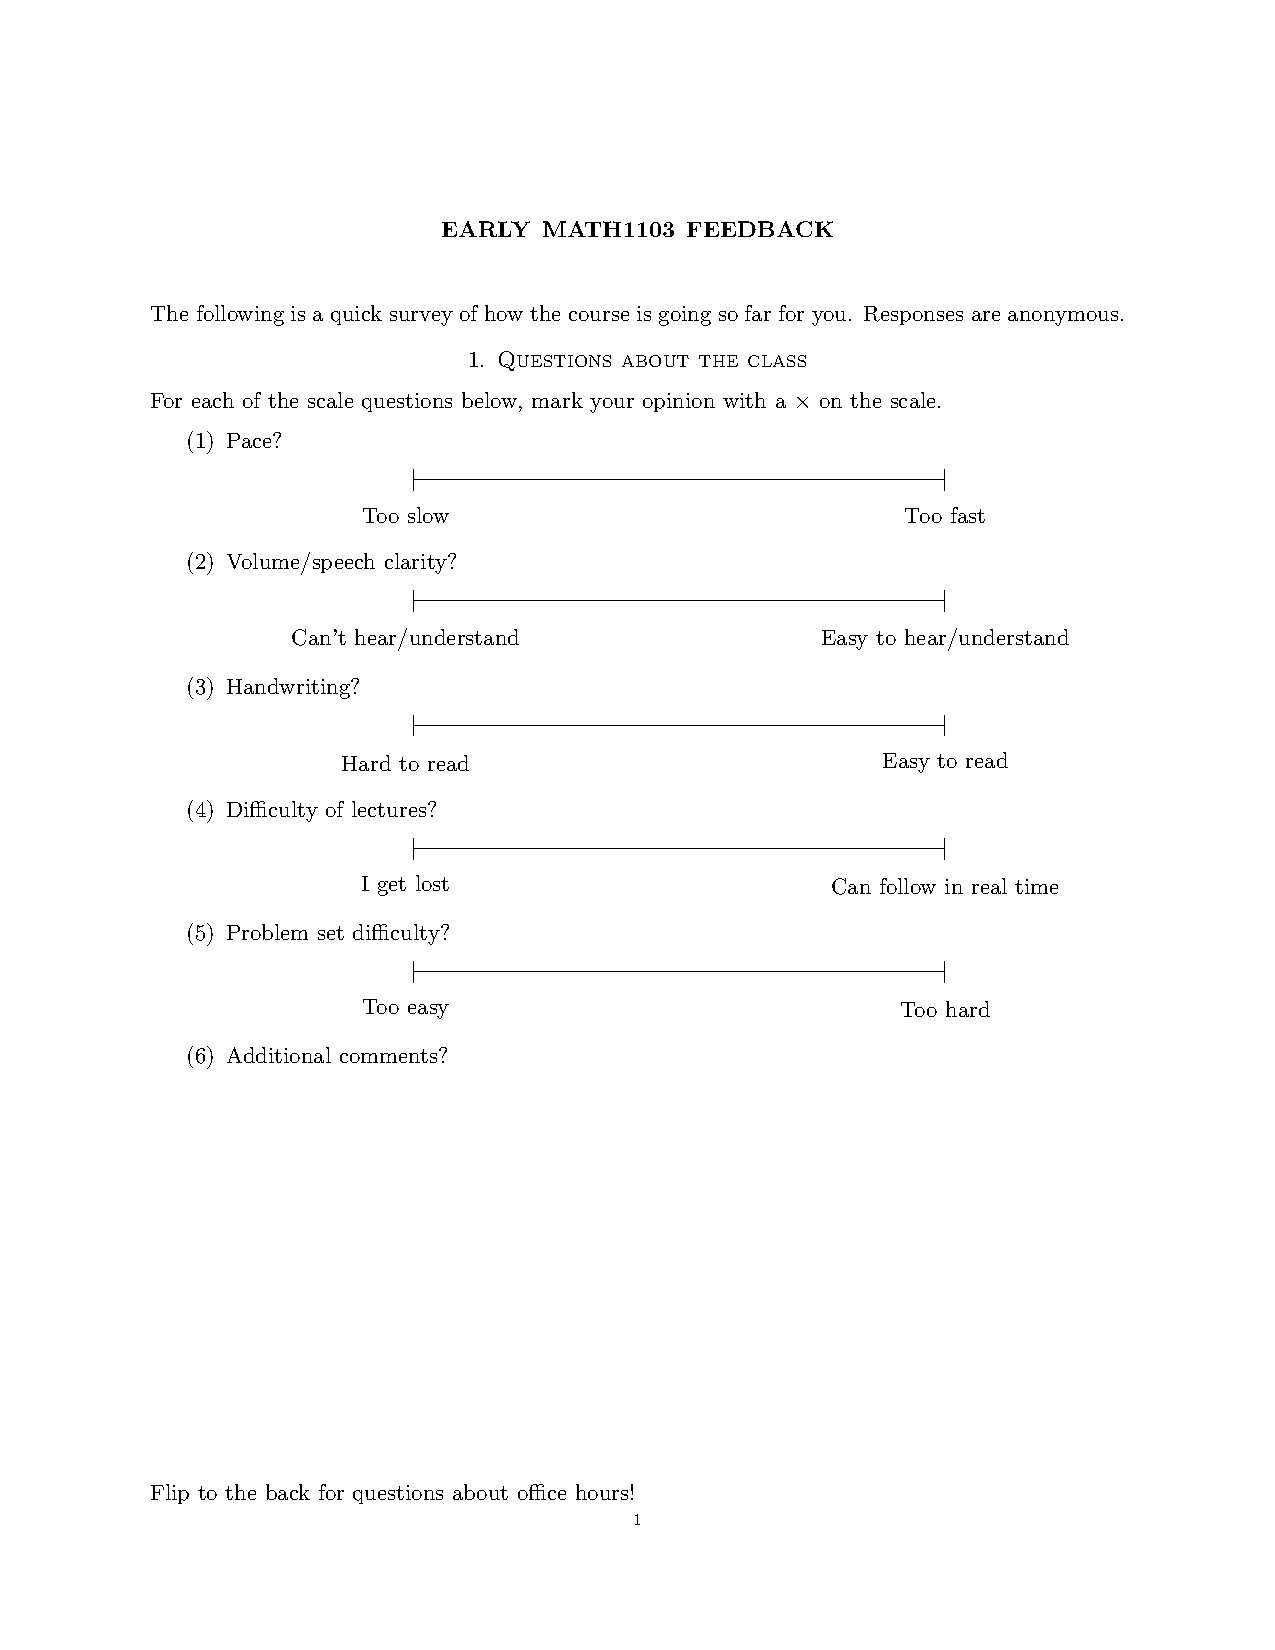
\includepdf[pages=-]{survey1.pdf}
\end{document}
